\documentclass[../main.tex]{subfiles}

\graphicspath{{../images/}}

\begin{document}
\pagestyle{fancy}
\lhead{Junseo Shin \& Jeremy Smith}
\rhead{Lab Notebook: Fourier Methods}
\chead{9/10/24}
\section{AM Radio Reception}

% chapter 3 & 11 
\subsection{Chapter 3: Modulated Waveforms - Amplitude Modulation}
\addcontentsline{toc}{subsection}{Chapter 3: Modulated Waveforms - Amplitude Modulation}

\paragraph*{Notes}
AM Modulation in a Nutshell: 

A high frequency ``carrier'' wave $f_c$ transports a lower frequency ``program'' content $f_p$, i.e.,
for a simple sinusoidal carrier wave the modulated signal is given by
\begin{align*}
    V(t) = [A(1 + \alpha\cos(2\pi f_p t))]\cos(2\pi f_c t)
\end{align*}
where $\alpha < 1$ is the modulation index. We can pretend that $[\;] = A(\;)$ is equivalent to the
amplitude of the modulated waveform, so this makes the amplitude vary over time between $A(1 - \alpha)$ and $A(1 + \alpha)$.
With some trig identities, we can rewrite this as
\begin{align*}
    V(t) = A\cos(2\pi f_c t) + \frac{A\alpha}{2}\cos(2\pi(f_c + f_p)t) + \frac{A\alpha}{2}\cos(2\pi(f_c - f_p)t)
\end{align*}
Thus the sum of three sinusodial waves with frequencies $f_c$, $f_c + f_p$, and $f_c - f_p$---i.e.,
the information content of an AM signal is contained within the sidebands of the carrier wave in the frequency domain.

\paragraph*{Exploration}
\begin{itemize}
    \item Carrier: 770 internal source---50 kHz, 1 V $\to$ Multipler module (MULT) input A
    \item Program: 33500B---2 kHz, 5 V $\to$ SUMMER module input B 
    \item DC VOLTAGE module 5 V $\to$ SUMMER input A
    \item SUMMER output $\to$ MULT input B
    \item MULT output $\to$ scope \& 770
\end{itemize}

% tabular fig2_1.png and fig2_2.png
\begin{figure*}[ht]
    \centering
    \begin{tabular}{cc}
        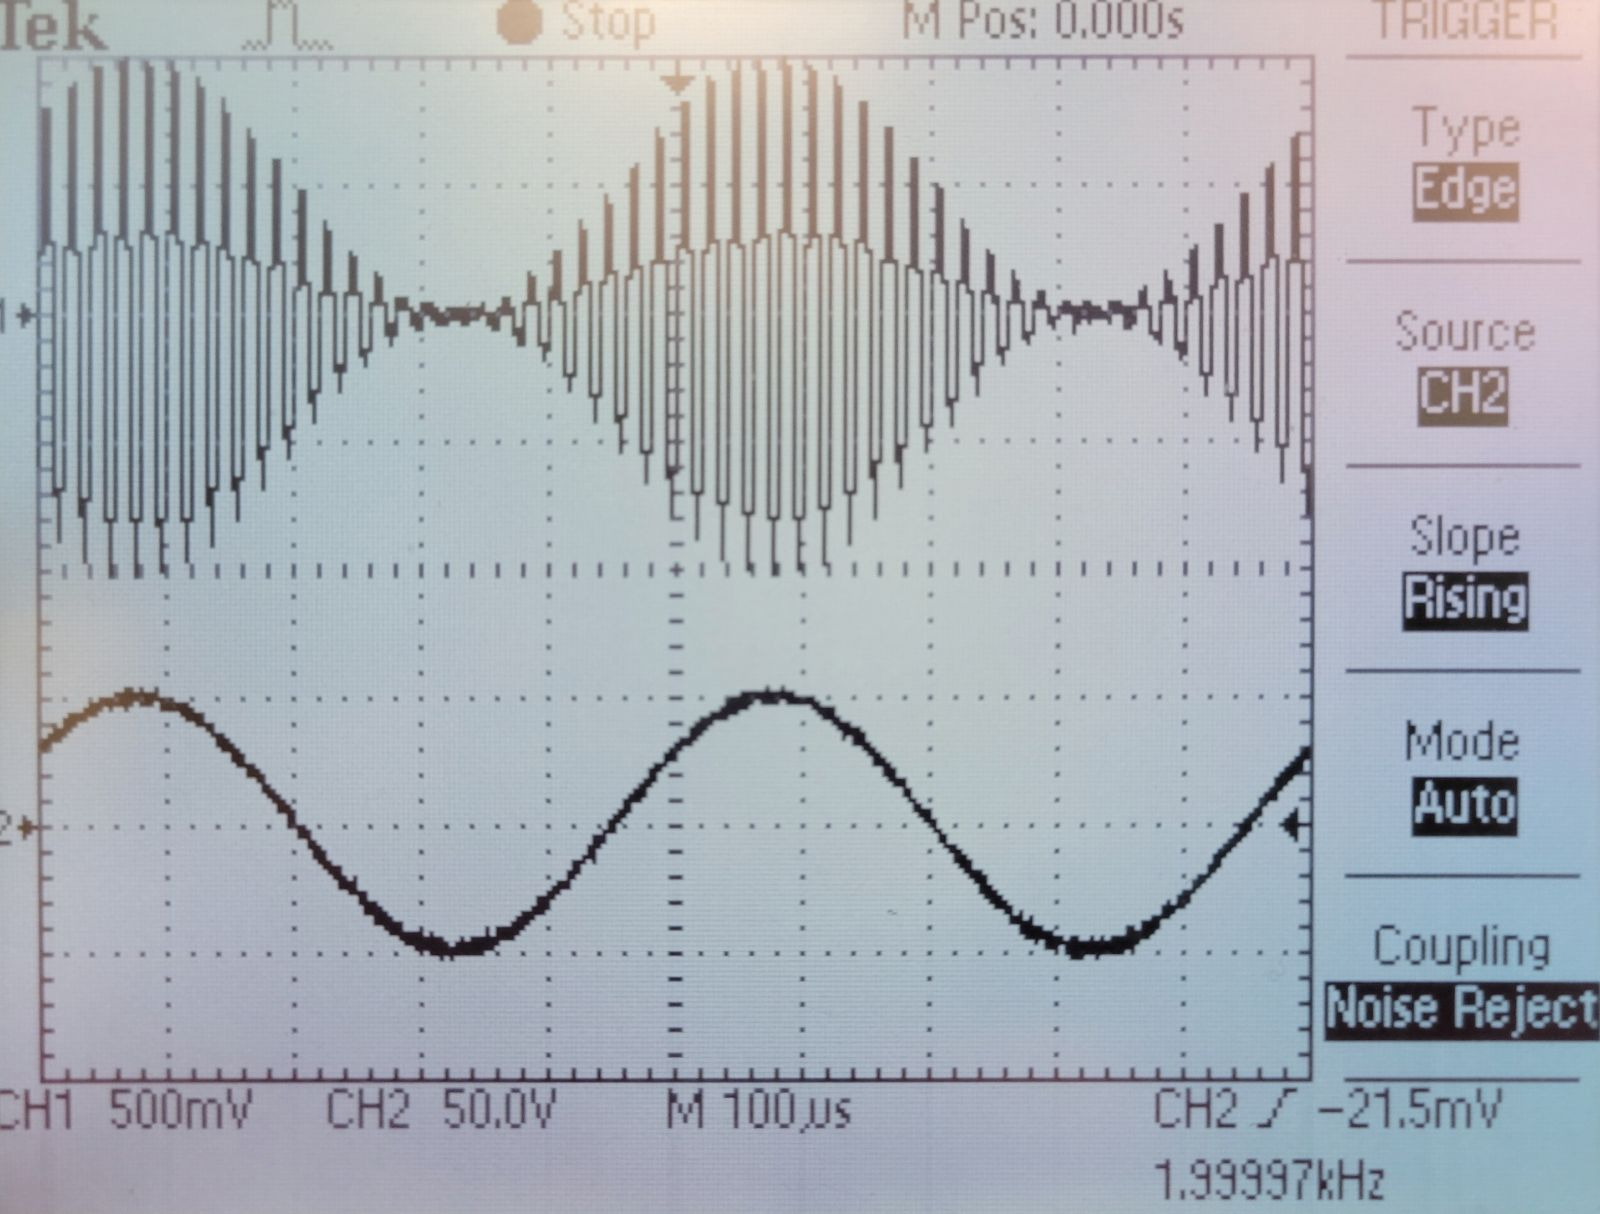
\includegraphics[width=0.45\textwidth]{fig2_1.png} & 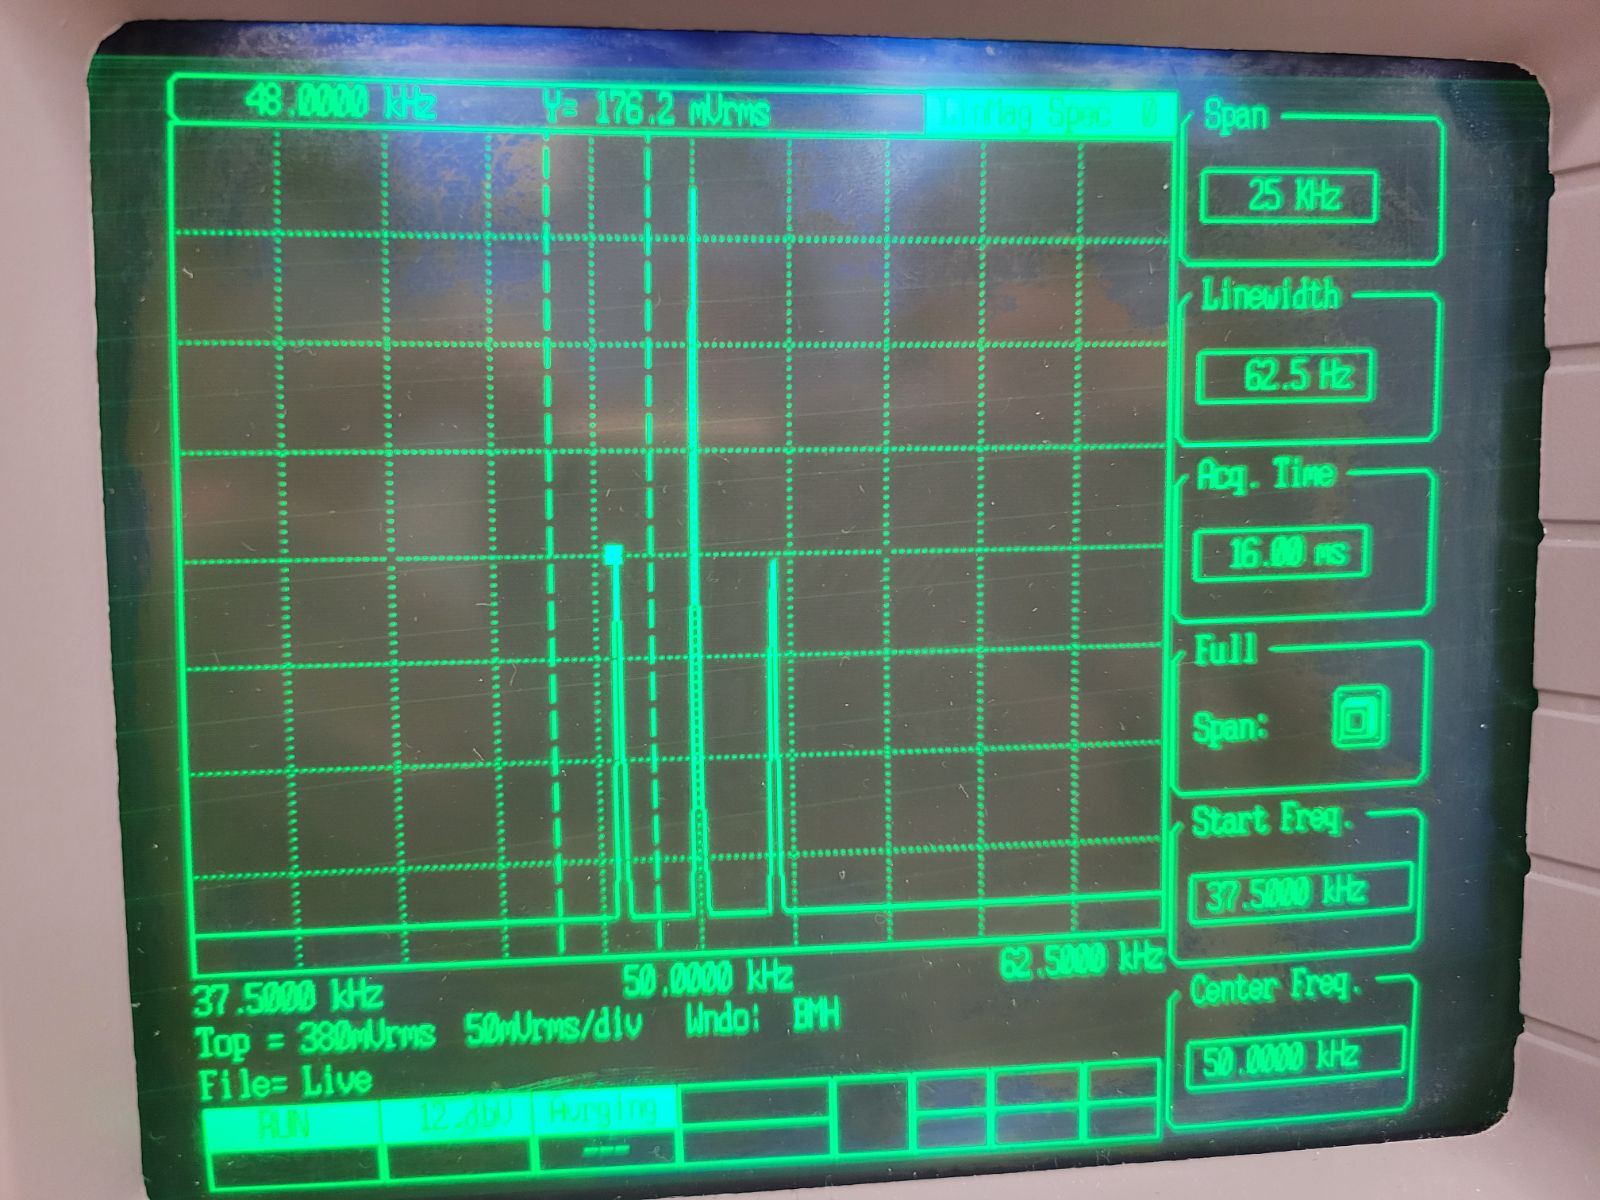
\includegraphics[width=0.45\textwidth]{fig2_2.png}
    \end{tabular}
    \captionsetup{width=0.8\textwidth}
    \caption{Scope (left) with bottom program content and 770 (right) view of AM Modulation of a 50 kHz carrier wave with a 2 kHz program wave.}
    \label{fig:am_modulation}
\end{figure*}

In Figure \ref{fig:am_modulation}, we see the scope and 770 view of the AM modulation of a 50 kHz carrier wave with a 2 kHz program wave.
The scope view shows familiar looking AM modulated waveform,
while the 770 clearly shows the carrier frequency at the center and the two sidebands which dictate the frequency of the program content.

\paragraph*{Changing content of the two waves}
\begin{itemize}
    \item Increase frequency of program content:
    \begin{itemize}
        \item The sidebands move further away from the carrier frequency just as the theory predicts $f_c \pm f_p$.
    \end{itemize}
    \item Change carrier frequency:
    \begin{itemize}
        \item Moves the 3 peak structure left or right (low freq and high freq respectively) on the 770 (Figure \ref{fig:2}).
        \item The envelope of the modulated waveform remains the same, but the inside oscillations increase as $f_c$ increases.
    \end{itemize}
    % fig2_3.png and fig2_4.png
    \begin{figure*}[ht]
        \centering
        \begin{tabular}{cc}
            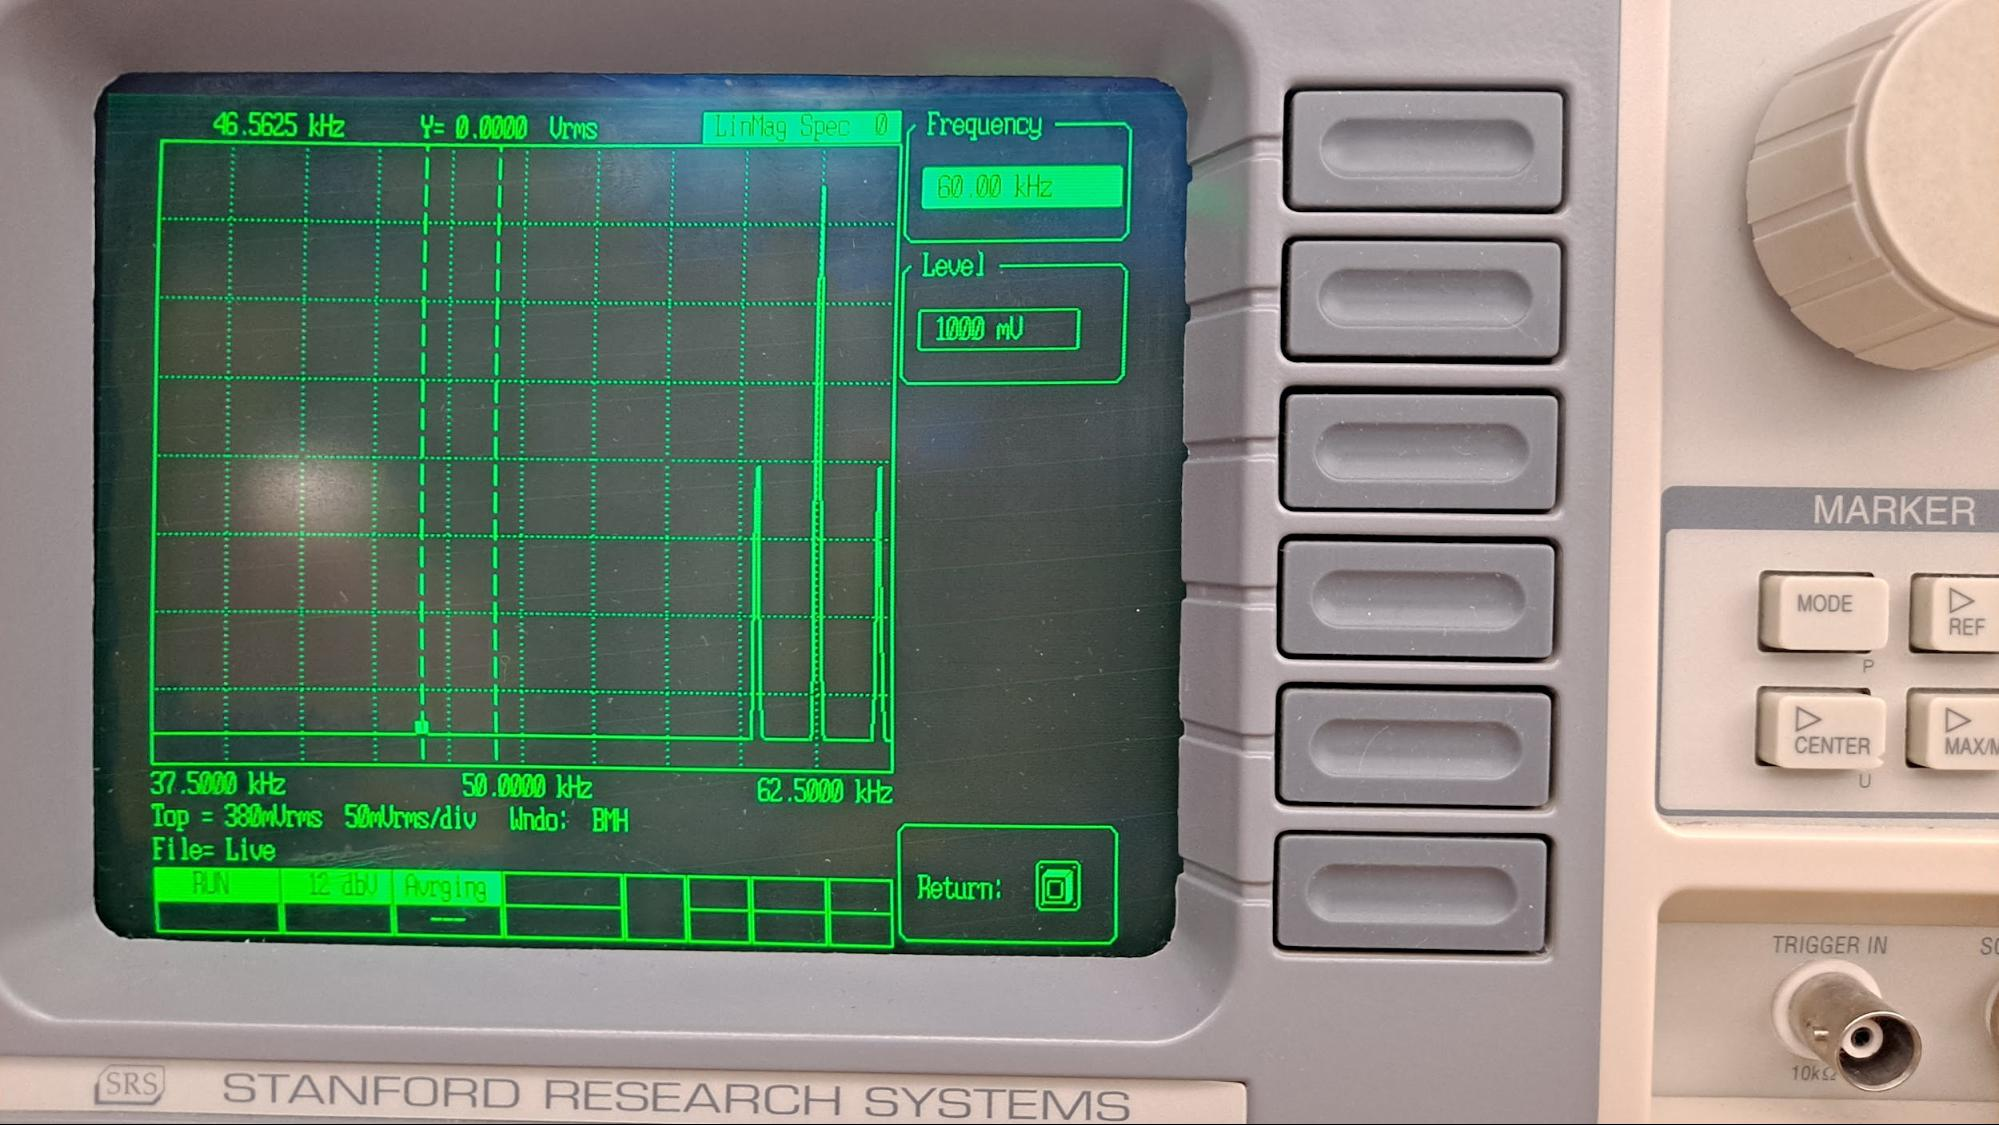
\includegraphics[width=0.45\textwidth]{fig2_3.png} & 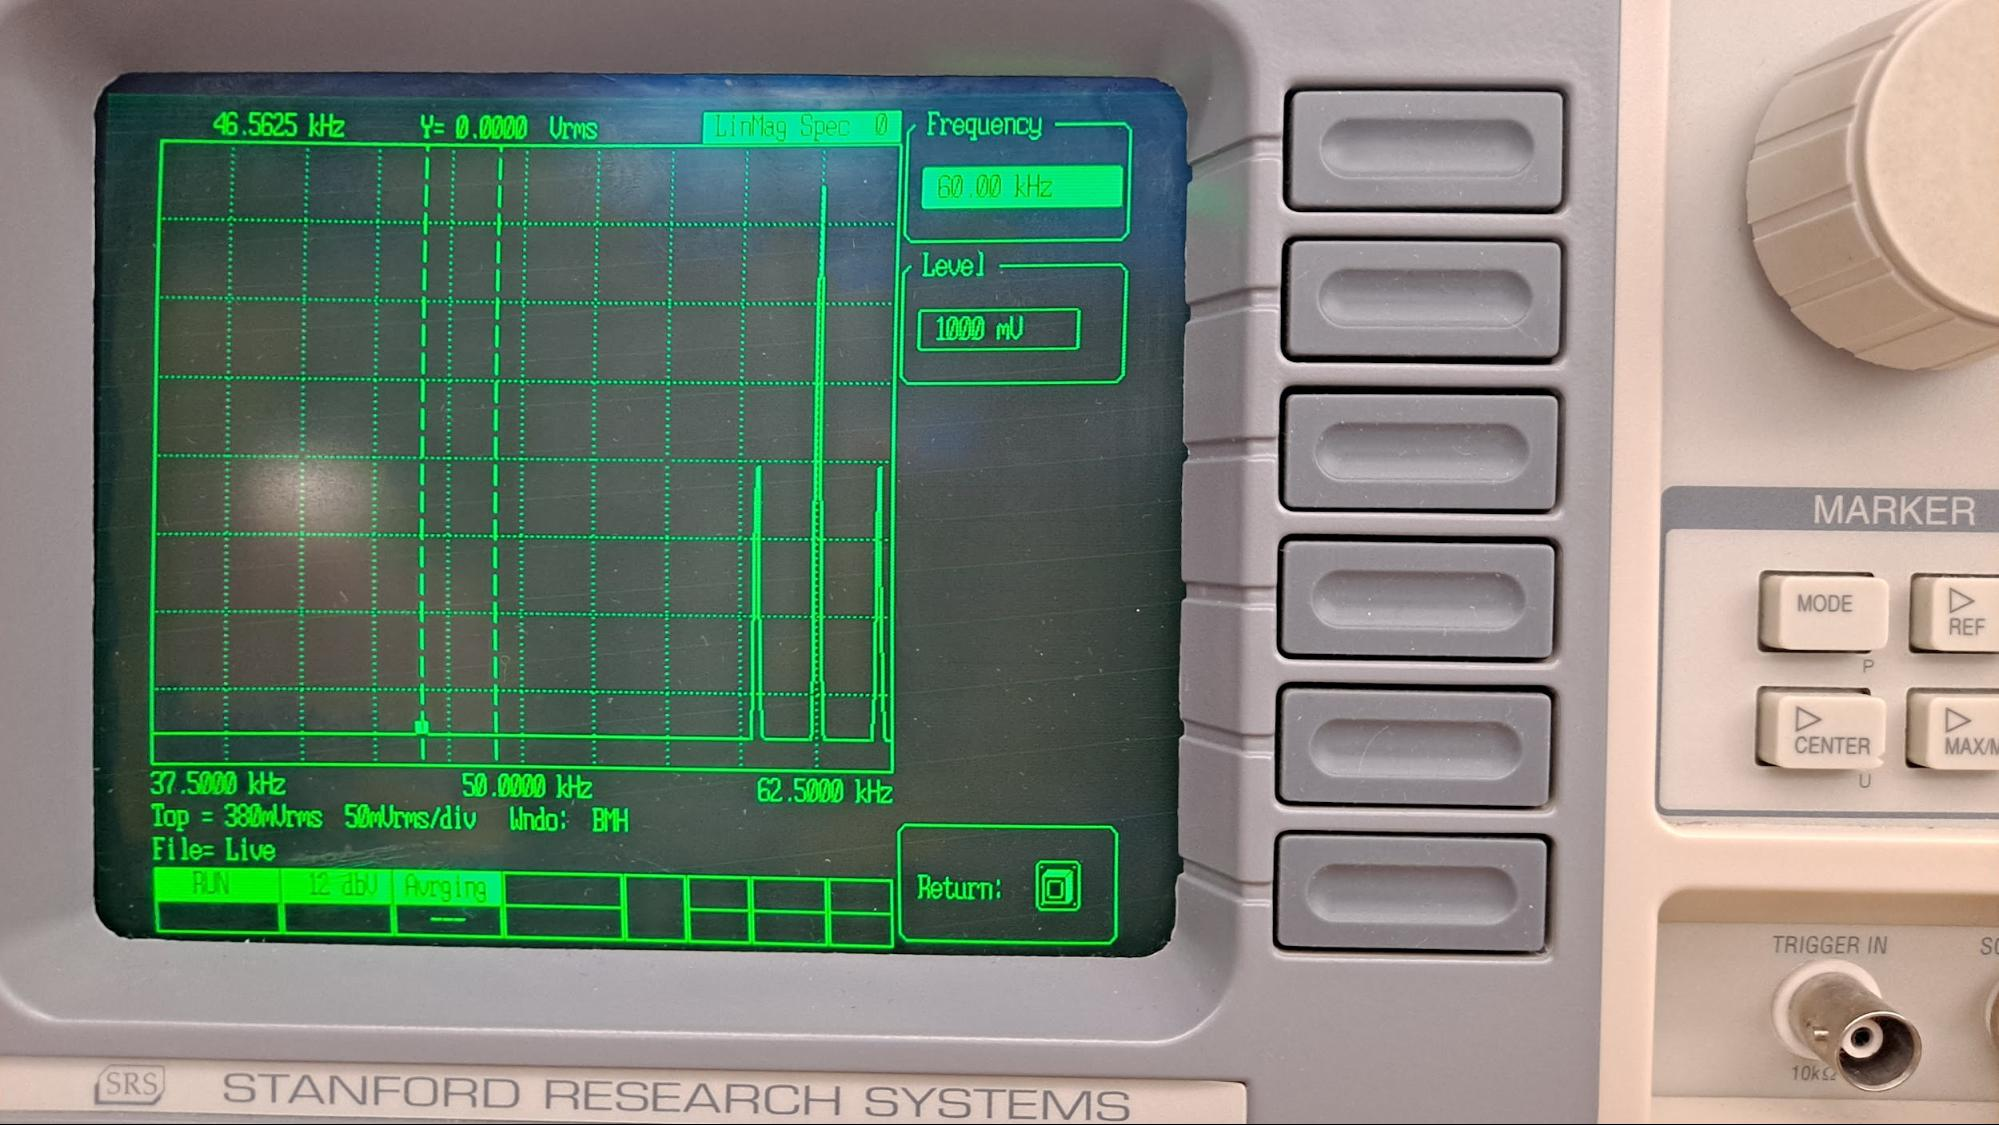
\includegraphics[width=0.45\textwidth]{fig2_4.png}
        \end{tabular}
        \captionsetup{width=0.8\textwidth}
        \caption{Increasing (right) and decreasing (left) program frequency.}
        \label{fig:2}
    \end{figure*}
    \item Program amplitude:
    \begin{itemize}
        \item Increasing the program amplitude increases the amplitude of the sidebands independent of the carrier amplitude (Fig. \ref{fig:3}).
    \end{itemize}
    % fig2_5.png
    \begin{figure}[ht]
        \centering
        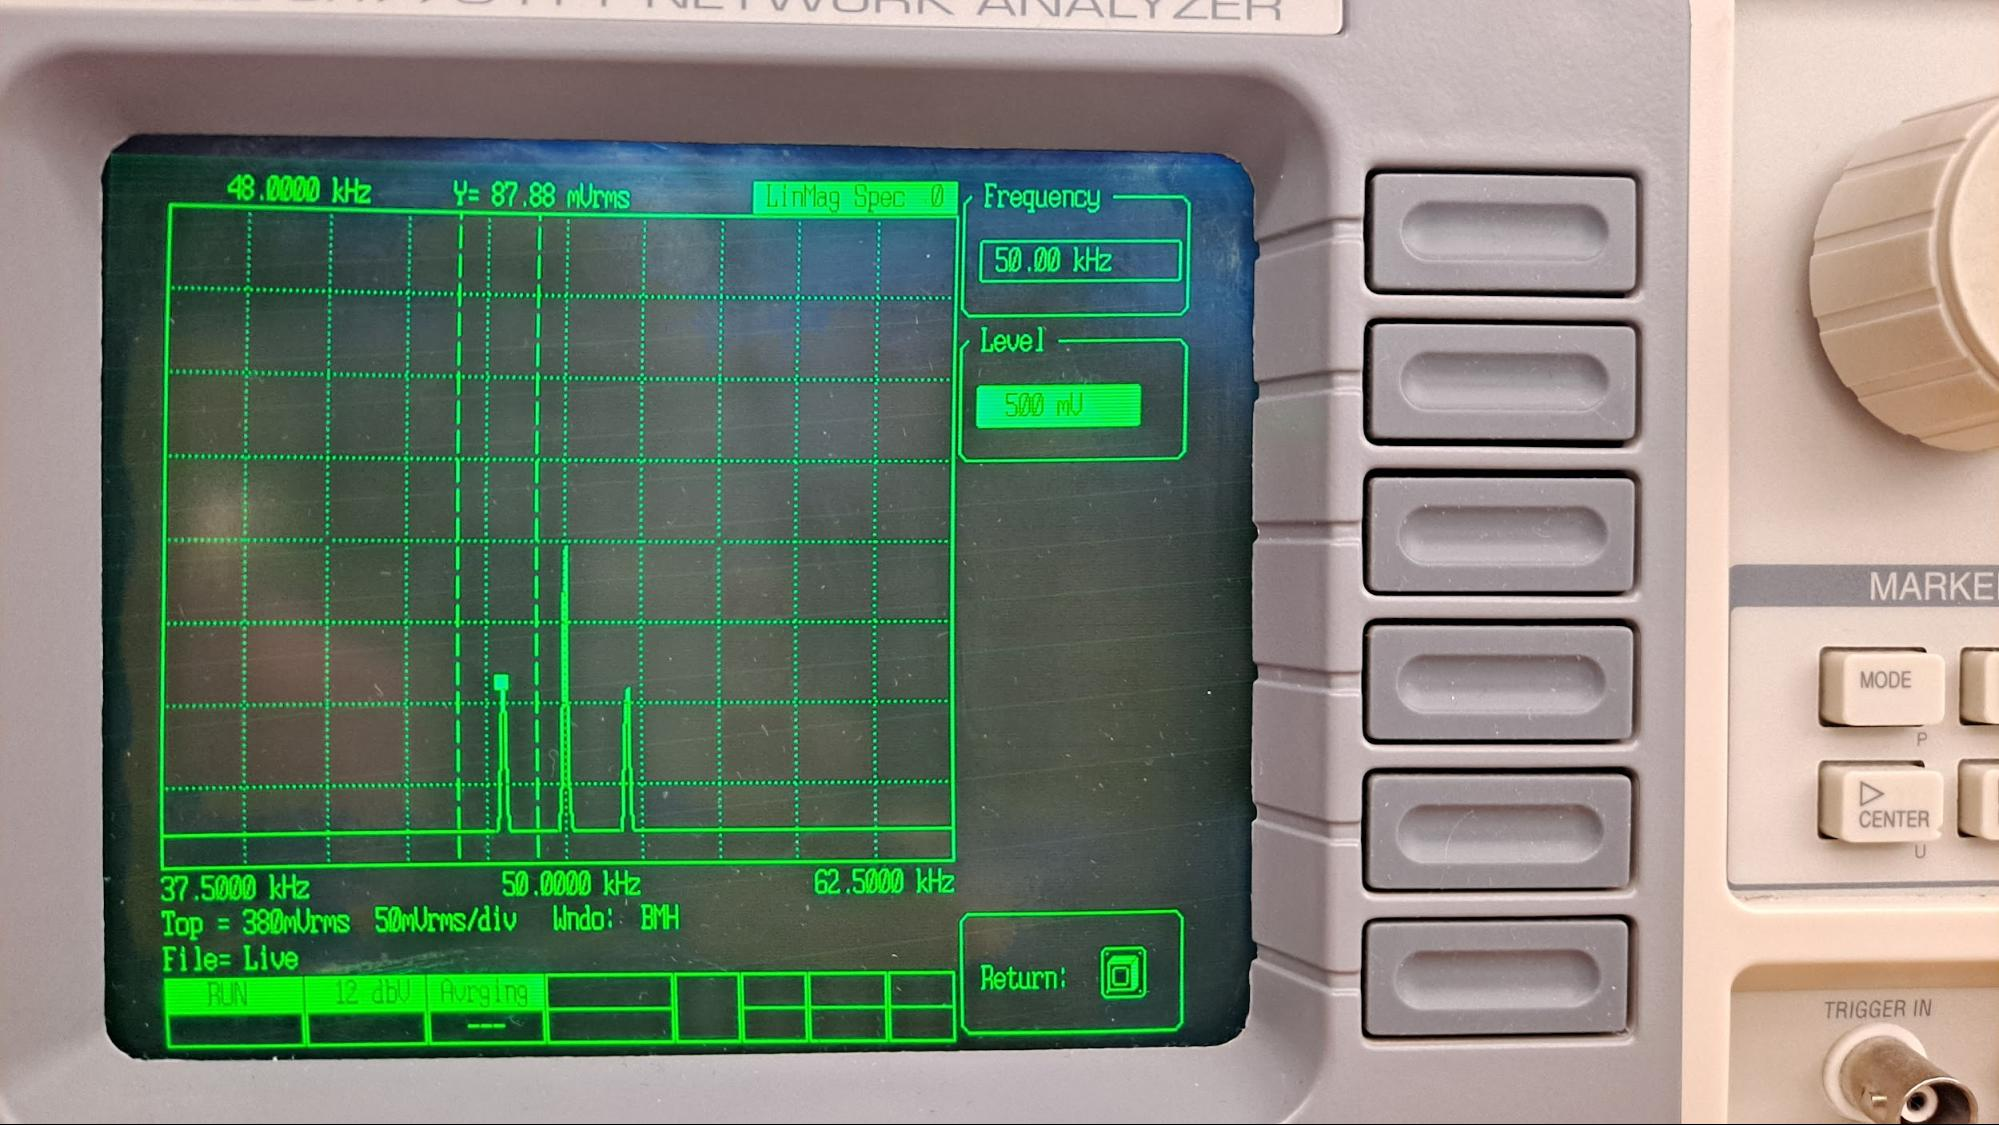
\includegraphics[width=0.45\textwidth]{fig2_5.png}
        \captionsetup{width=0.8\textwidth}
        \caption{Decreasing program amplitude.}
        \label{fig:3}
    \end{figure}
    \item Carrier amplitude:
    \begin{itemize}
        \item Increasing the carrier amplitude increases the amplitude of the carrier wave independent of the program amplitude (Fig. \ref{fig:4}).
    \end{itemize}
    % fig2_6.png and fig2_7.png
    \begin{figure*}[ht]
        \centering
        \begin{tabular}{cc}
            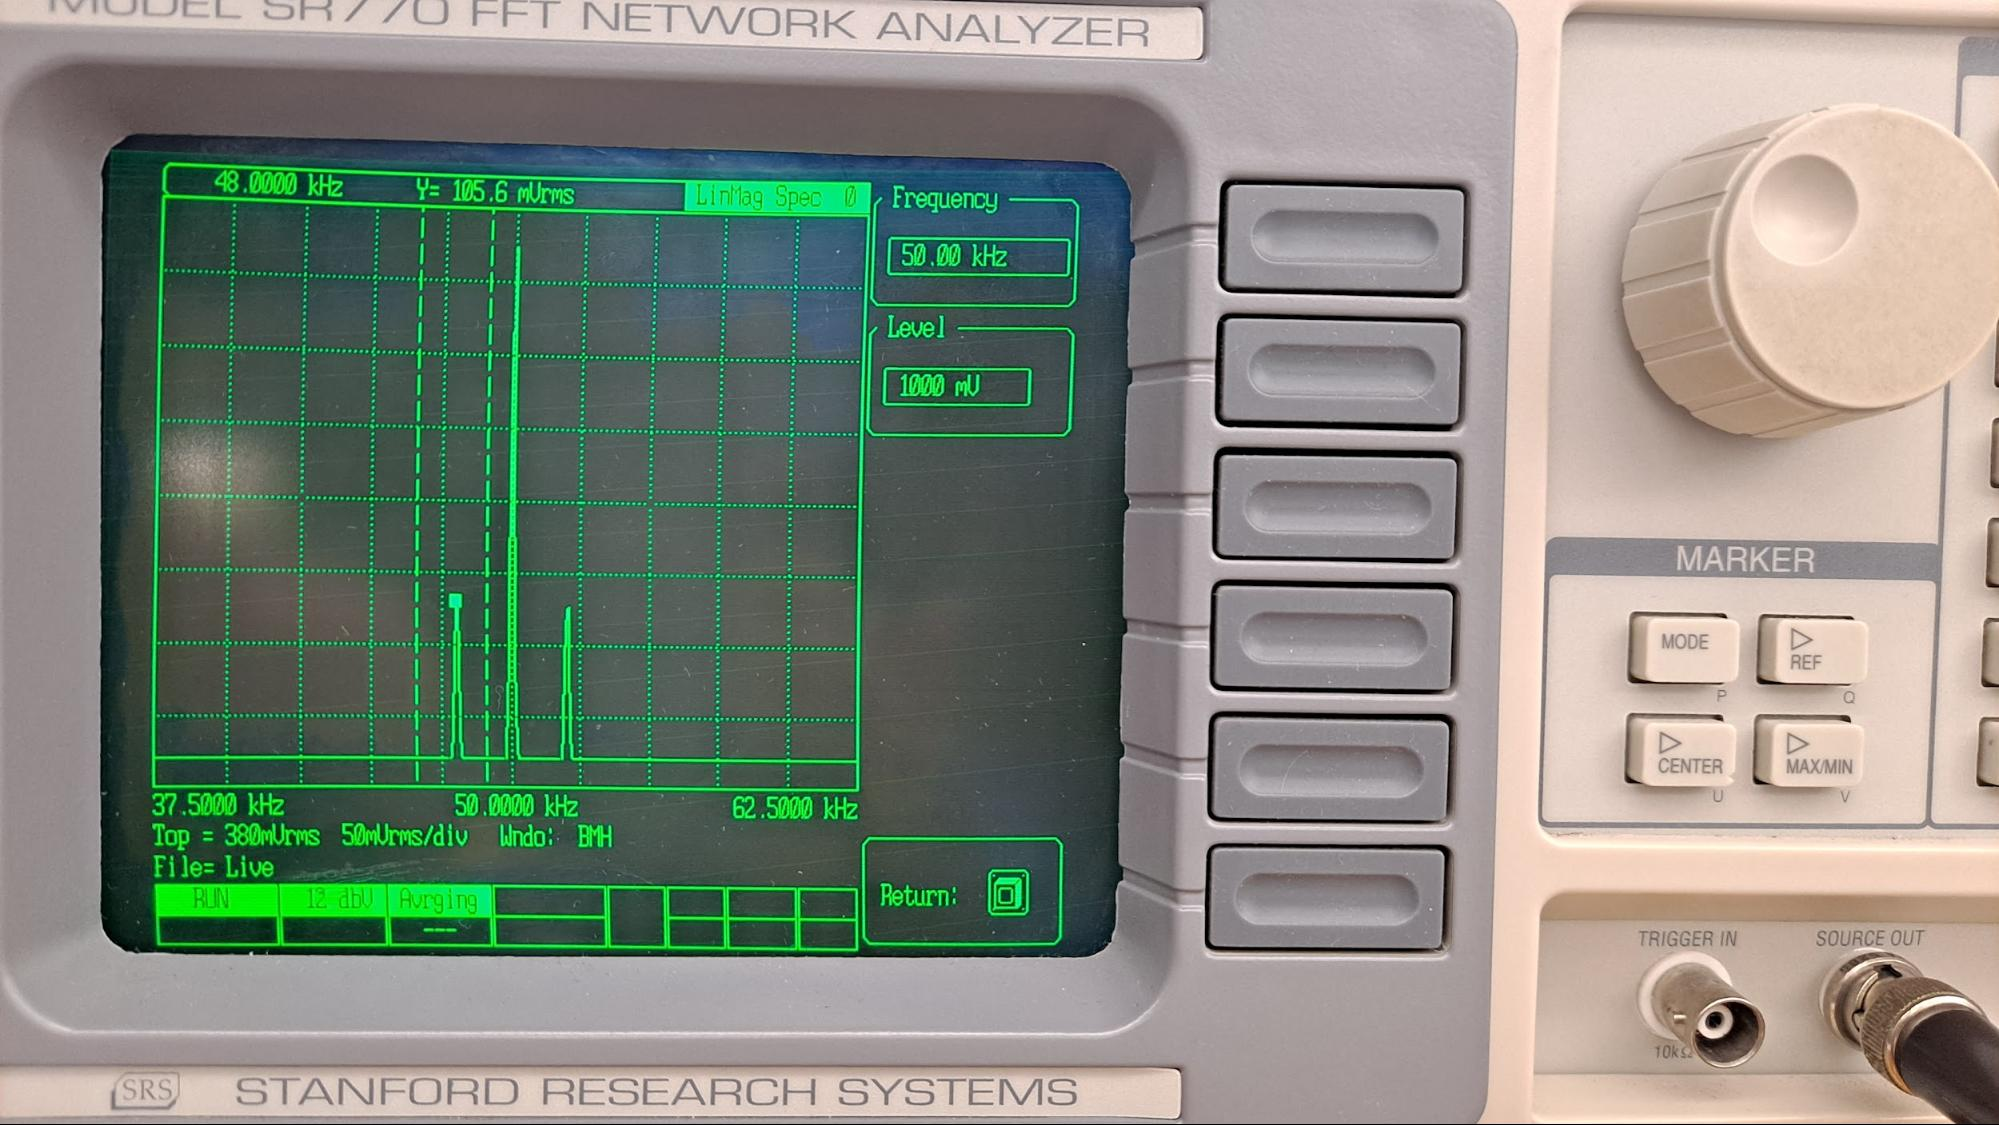
\includegraphics[width=0.45\textwidth]{fig2_6.png} & 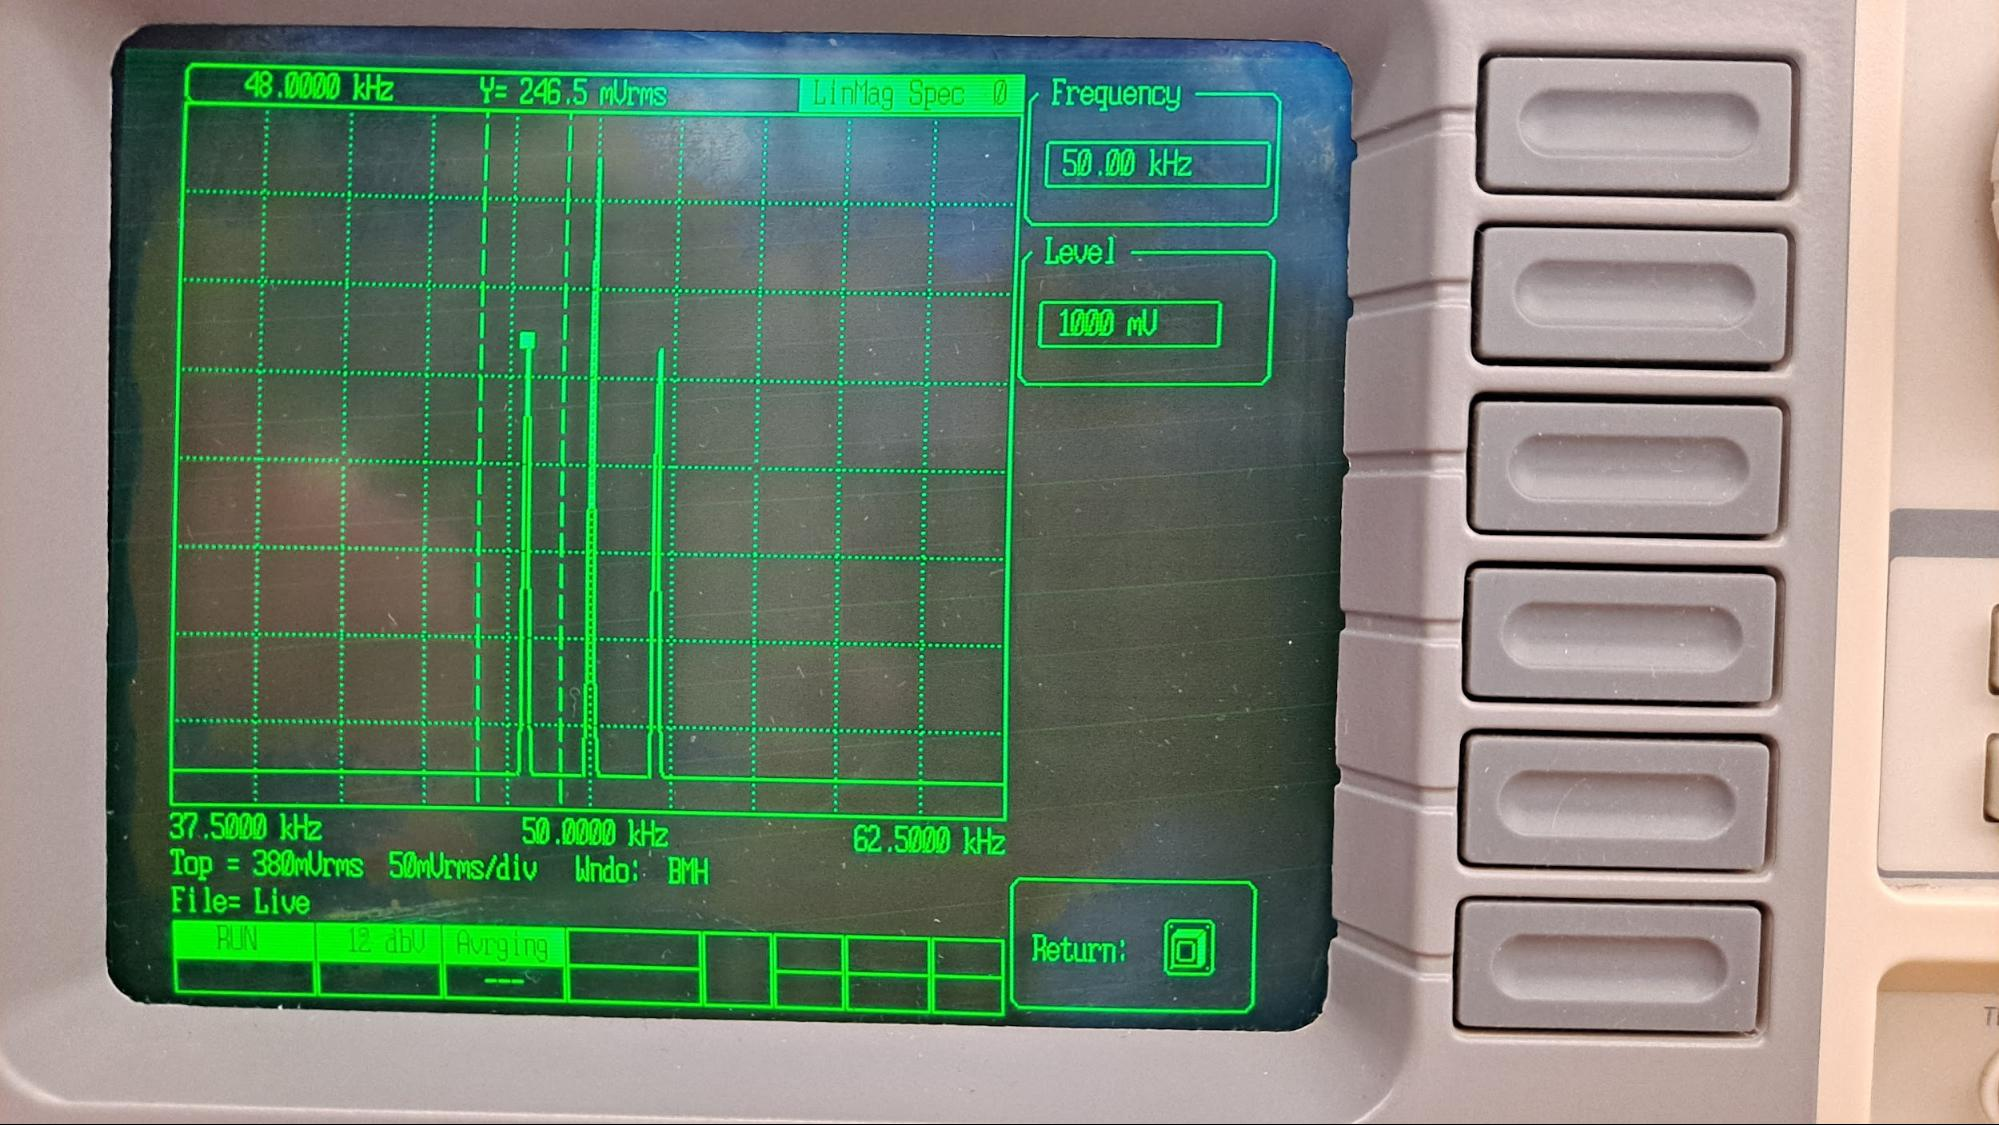
\includegraphics[width=0.45\textwidth]{fig2_7.png}
        \end{tabular}
        \captionsetup{width=0.8\textwidth}
        \caption{Increasing (right) and decreasing (left) carrier frequency.}
        \label{fig:4}
    \end{figure*}
    \item Program content to square wave:
    \begin{itemize}
        \item There are multiple sidebands at odd multiples of the program frequency.
    \end{itemize}
    % fig2_8.png and fig2_9.png
    \begin{figure*}[ht]
        \centering
        \begin{tabular}{cc}
            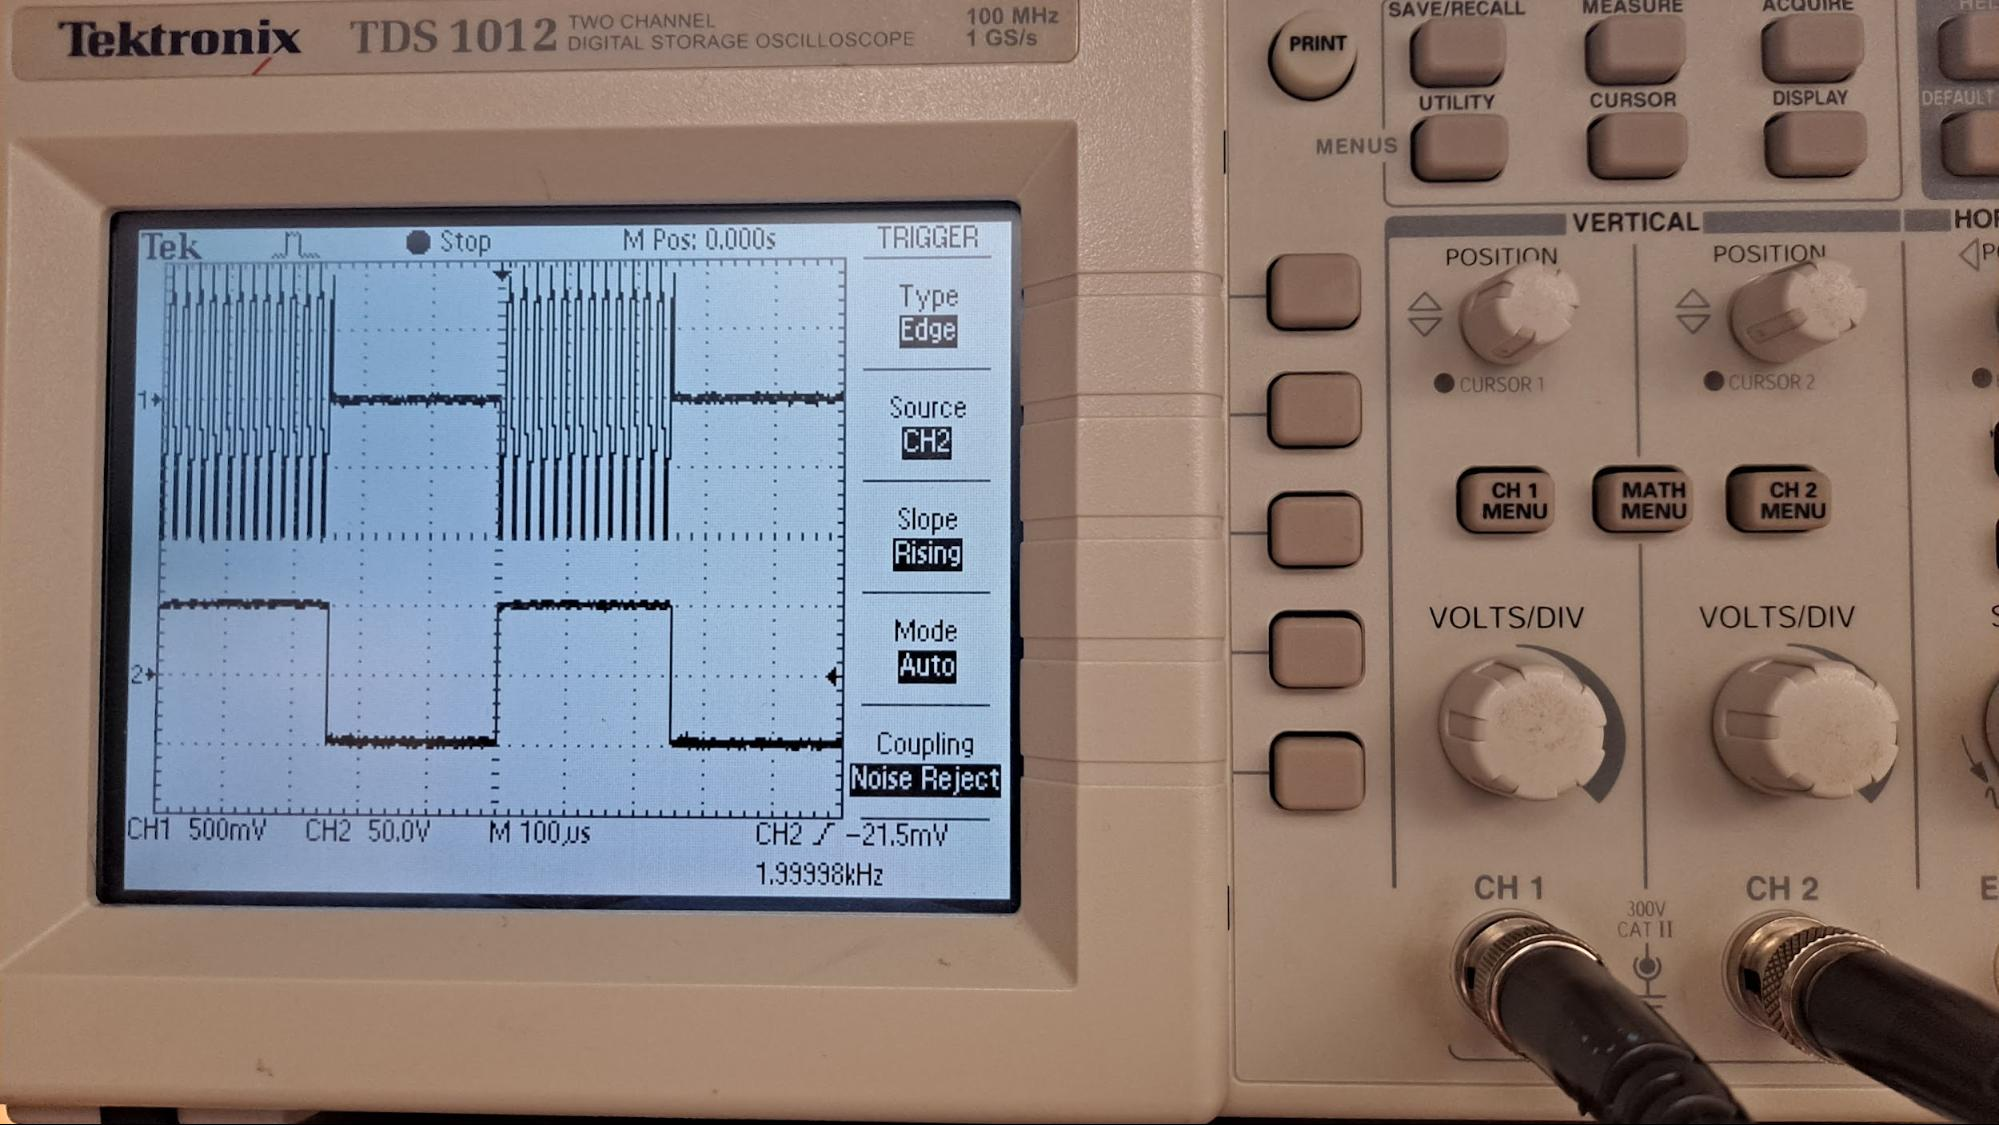
\includegraphics[width=0.45\textwidth]{fig2_8.png} & 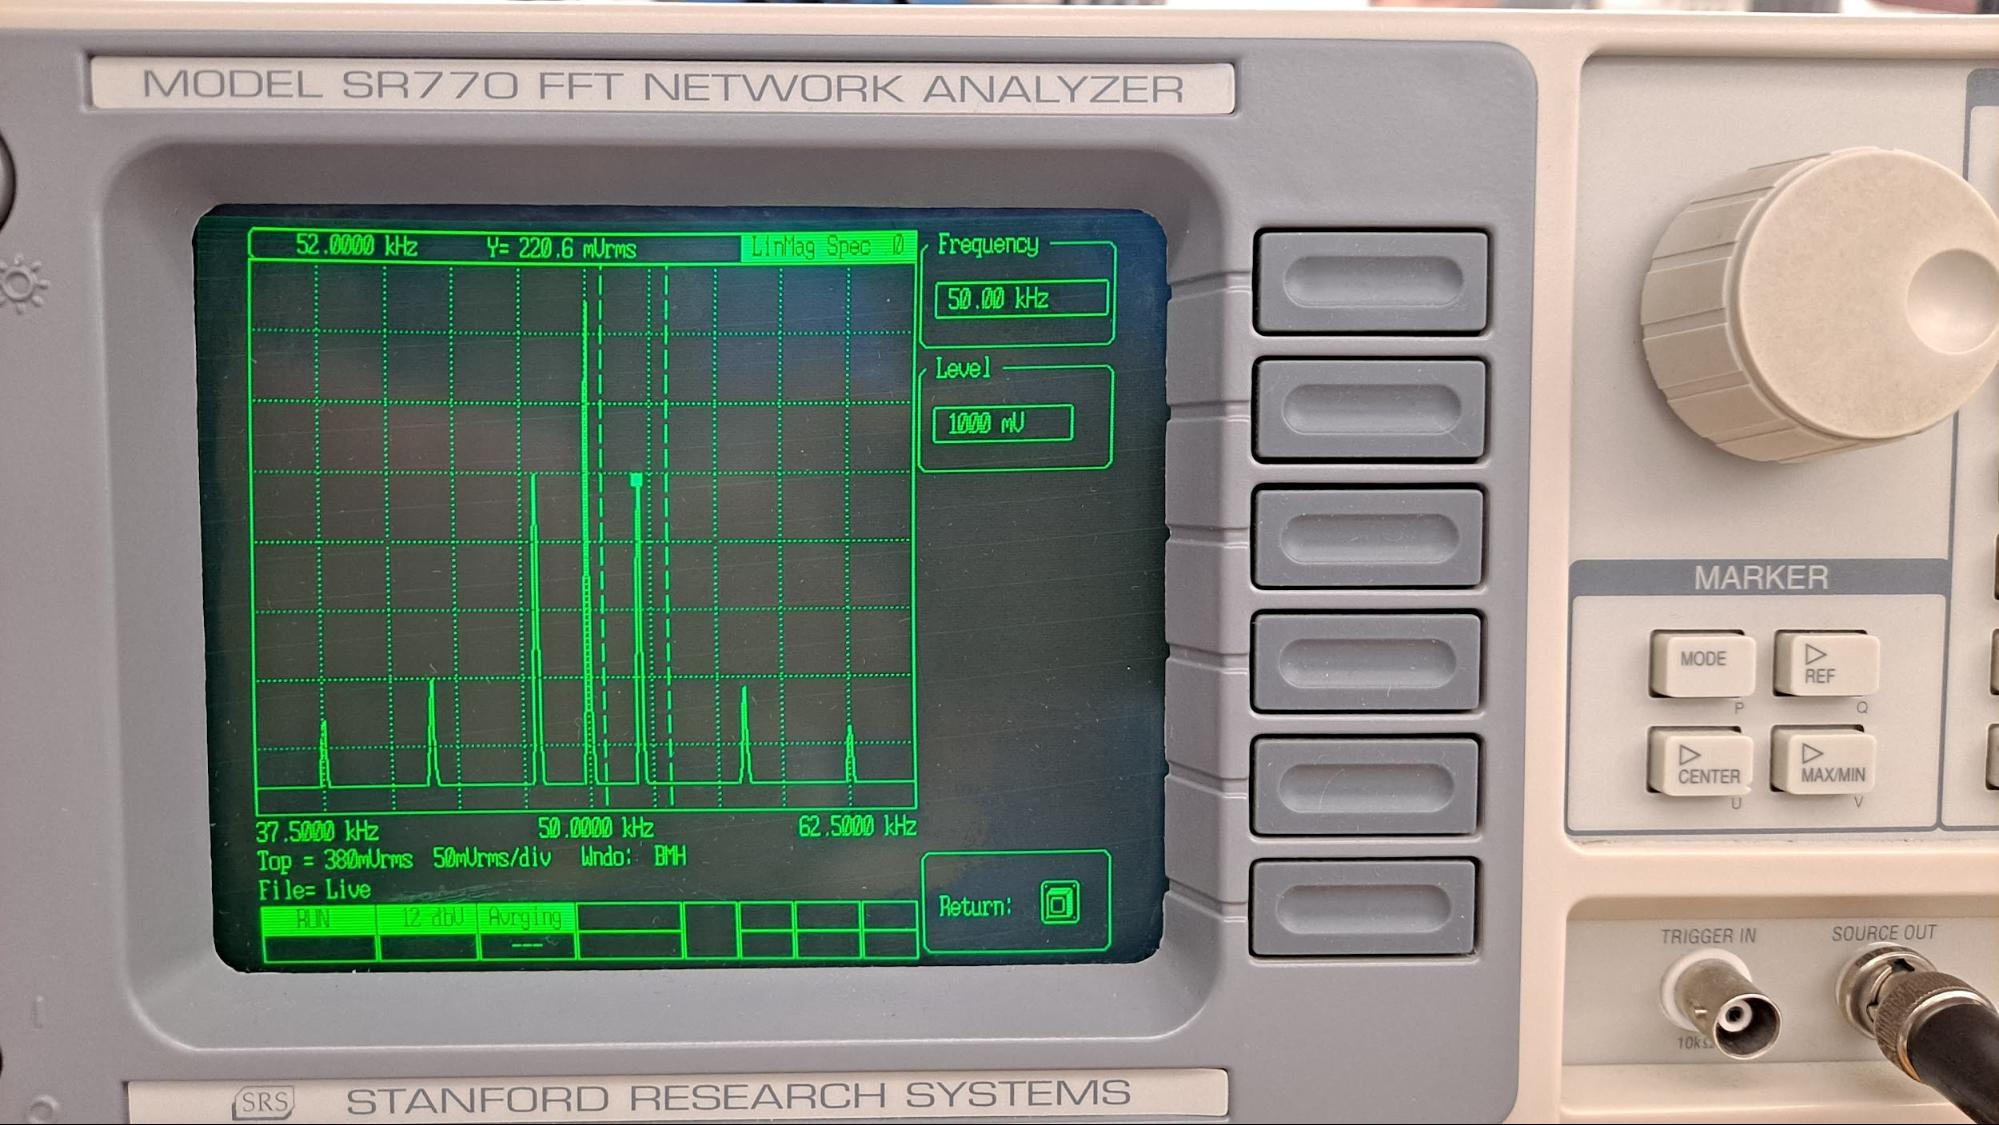
\includegraphics[width=0.45\textwidth]{fig2_9.png}
        \end{tabular}
        \captionsetup{width=0.8\textwidth}
        \caption{Scope (left) with program content in the bottom and 770 (right) view of AM Modulation of a 50 kHz carrier wave with a 2 kHz square wave program wave.}
        \label{fig:5}
    \end{figure*}
\end{itemize}

\paragraph*{Why $\alpha < 1$?}
The multiplier ouputs a scaled product of the two input signals
\begin{align*}
    V_{\text{out}} = \frac{V_A V_B}{10}
\end{align*}
for inputs with voltage $\pm 10$ V, and frequency lower than $1$ MHz. Thus for $5$ V DC input from the summer with the program signal gives
\begin{align*}
    V_{\text{out}} &= (5 V + P \cos(2\pi f_p t)) (A \cos(2\pi f_c t)) / 10 \\
    &= \frac{5A}{10} V \qt(1 + \frac{P}{5 V} \cos(2\pi f_p t)\qt) \cos(2\pi f_c t)
\end{align*}
So the waveform has a modulation index $\alpha = \frac{P}{5 V}$. In our first case (Fig. \ref{fig:am_modulation}), $P = 5 V$ so $\alpha = 1$,
Here the scope clearly shows the two distinct frequencies that make up the AM waveform---i.e., the envelope matches the program content shown simultaneously below,
and the carrier frequency is resolved in the small oscillations within the envelope.

When we increase $\alpha \to 2$ (Fig. ref here), the program content is overmodulated or \textit{distorted} which makes it hard to extract
out the program content from the modulated waveform. 


\subsection*{Chapter 11: AM Radio Reception}
\addcontentsline{toc}{subsection}{Chapter 11: AM Radio Reception}

\paragraph*{Notes}
\begin{itemize}
    \item Since AM radio signals are roughly 540-1600 kHz, i.e., 500-200 m wavelength, the EM waves are pretty uniform and can be received by our simple electrical wire antenna connected to an LC-resonant circuit. 
    \item The LC-resonant slighly tunes the frequency range into a narrow band of frequencies, which can be changed by adjusting the number of inductors we put in series (Fig. \ref{fig:6}).
    % fig2_11.png
    \begin{figure*}[ht]
        \centering
        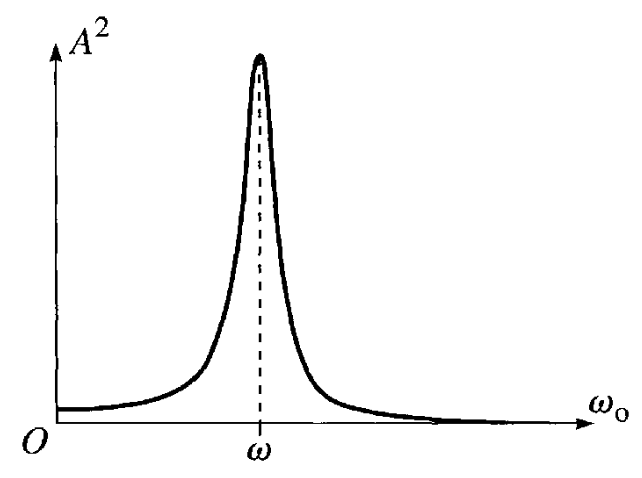
\includegraphics[width=0.45\textwidth]{fig2_11.png}
        \captionsetup{width=0.8\textwidth}
        \caption{Resonant frequency of RLC circuit (Taylor, Classical Mechanics). Our circuit has a broad resonance (rather than sharp) which will receive a band full of AM stations.}
        \label{fig:7}
    \end{figure*}
    \item Downcoversion: Before we narrow the frequency search range, we can first use downconversion to bring the high frequency AM signals to a lower frequency range provided by the High-Frequency (HF) Mixer module.
    \begin{itemize}
        \item Local-oscillator (LO) source: Using the 33500B, we set the LO frequency so that the difference between the LO and the AM signal is in the range of our 770 (100 kHz). 
        e.g., for target radio station (RF) $850$ kHz, setting the LO to $770$ or $930$ kHz will output a $80$ kHz difference frequency from the HF mixer. It will also ouput and sum \& difference frequencies from other radio stations which we must filter with the IF output.
        \item IF Filter: To create a fixed pass band that only allows the a narrow range of difference frequencies to pass through.
    \end{itemize}
\end{itemize}

%fig2_10.png
\begin{figure*}[ht]
    \centering
    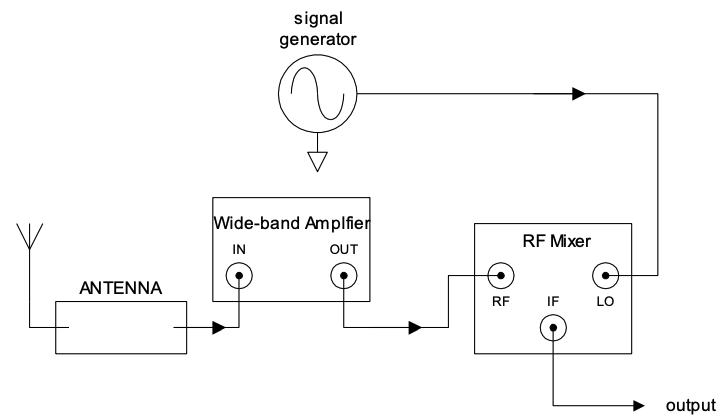
\includegraphics[width=0.45\textwidth]{fig2_10.png}
    \captionsetup{width=0.8\textwidth}
    \caption{AM Radio Reception setup.}
    \label{fig:6}
\end{figure*}

\paragraph*{Experiment:} Finding Radio Stations
\begin{itemize}
    \item First note a near by radio station we can pick up from St. Louis \href{https://radio-locator.com/cgi-bin/locate?select=city&city=saint+louis&state=mo&x=0&y=0}{(Radio Station List)}. e.g. KFUO 850 kHz.
    \item Set three inductors in series on the radio antenna circuit
    \item Radio antenna circuit OUPUT $\to$ Wideband Amp (10x) or until the signal is visible on the scope
    \item Wideband Amp OUTPUT $\to$ HF Mixer INPUT RF
    \item 33500B 0.7 to 1.1 V with difference frequency of 80 kHz OUTPUT $\to$ HF Mixer INPUT LO
    \item IF OUT $\to$ Filter Module 80 kHz; 8 Gain
    \item Filter OUT $\to$ scope \& 770 and note the visualized signal
    \item Tune the LO frequency to get a strong signal
    \item De-modulate the signal by tuning the LO frequency \textit{exactly} to the Radio station frequency (carrier freq) tjnhe zero beat frequency, e.g., 
\end{itemize}

\end{document}